overle%
% teil2.tex -- Beispiel-File für teil2 
%
% (c) 2020 Prof Dr Andreas Müller, Hochschule Rapperswil
%
% !TEX root = ../../buch.tex
% !TEX encoding = UTF-8
%
\section{Helmholtz-Zerlegung für $\mathbb{R}^3$
\label{helmholtz:section:teil2}}
\kopfrechts{Teil 2}

Die Grundidee der Helmholtz-Zerlegung besteht darin, dass ein glattes (differenziebares) Vektorfeld $\mathbf{F}$, welches unendlich schnell genug abfällt, in zwei orthogonale Komponenten zerlegenlässt. Und zwar in ein eindeutig wirbelfreien (irrotationalen) Teil und einen quellenfreien (solenoidalen) Teil. Diese Zerlegung spiegelt die physikalischen Eigenschaften des Vektorfeldes wider und ist insbesondere in der Akustik, Strömungsmechanik und Elektrodynamik von zentraler Bedeutung.

\begin{equation}
\underbrace{\mathbf{F}}_{\text{zu zerlegendes Vektorfeld}} =  \underbrace{-\nabla \Phi}_{Skalarpotential} + \underbrace{\nabla \times \mathbf{\Psi}}_{Vektorpotential}
\label{helmholtz:equationAllgemein}
\end{equation}

Die physikalische Bedeutung dieser Komponenten lässt sich wie folgt beschreiben:

\begin{itemize}
\item Der erste Term $ \nabla \Phi $ ist wirbelfrei (irrotational), da Rotation verschwindet ($\nabla \times (-\nabla \Phi) = 0$) 
\begin{itemize}
\item Dieser Anteil hat keine Rotation: $\nabla \times (-\nabla \Phi) = 0$
\item Die Feldlinien verlaufen strahlenförmig von Quellen zu Senken
\begin{table}[h]
\centering
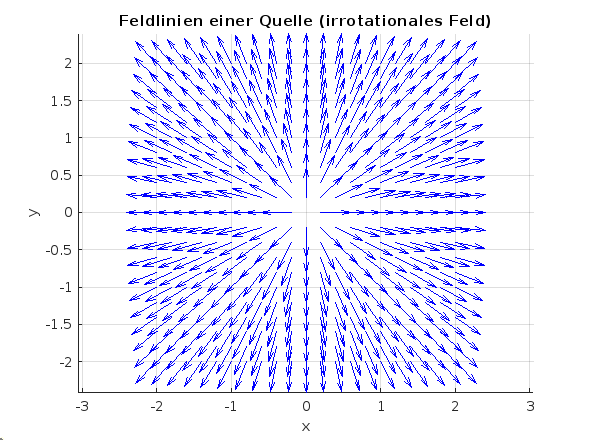
\includegraphics[scale=0.3]{papers/helmholtz/images/Quelle.png}
\caption{Quelle}
\label{fig:quelle}
\end{table}
 \begin{table}[h]
        \centering
        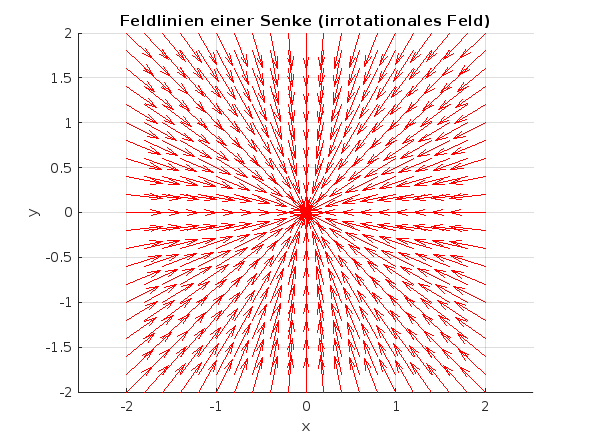
\includegraphics[scale=0.3]{papers/helmholtz/images/Senke.png} 
        \caption{Senke}
        \label{fig:senke}
\end{table}

\end{itemize}
\item Der zweite Term $\nabla \times \mathbf{\Psi}$ hat gemäss der Definition immer Divergenz null ($\nabla \cdot (\nabla \times \mathbf{\Psi}) = 0$) und wird auch solenoidal (quellenfrei) genannt. \newline
\begin{itemize}
\item Dieser Anteil hat keine Divergenz:$\nabla \cdot (\nabla \times \mathbf{\Psi}) = 0$
\item Die Feldlinien bilden geschlossene Schleifen (ähnlich einem Magnetfeld).
\end{itemize}
\end{itemize}

\begin{table}[h]
\centering
\begin{tabular}[h]{l|l|l|l}
\hline
zu zerlegende Vektorfeld & $\mathbf{F}$ & & \\
\hline 
skalares Potential & $\Phi $ & $\nabla \times (-\nabla \Phi) = 0$ & wirbelfrei\\
\hline
Vektorpotential & $\mathbf{\Psi}$ & $\nabla \cdot (\nabla \times \mathbf{\Psi}) = 0$ & quellenfrei\\
\hline
\end{tabular}\newline
\caption{Übersicht der Helmholtz-Zerlegung}
\end{table}

Um die Zerlegung anwenden zu können, müssen die Potentiale $\Phi $ und $\mathbf{\Psi}$ berechnet werden. Dies kann auf verschiedene Methoden gemacht werden abhängig von den Ranbedingungen.

\subsubsection{Nachweis der Wirbelfreiheit des irrotationalen Anteils}
Sei $\Phi$ ein zweimal stetig differenzierbares Skalarfeld.

\begin{enumerate}
    \item \textbf{Zuerst wird der Gradient $\nabla\Phi$ berechnet:}
    $$
    \nabla \Phi =
    \begin{pmatrix}
        \frac{\partial \Phi}{\partial x} \\
        \frac{\partial \Phi}{\partial y} \\
        \frac{\partial \Phi}{\partial z}
    \end{pmatrix}
    $$

    \item \textbf{Nun die Rotation dieses Gradientenfeldes:}
    
    Die Definitionsformel der Rotation $\nabla \times F$ auf den Gradientenvektor anwenden.
    $$
    \nabla \times (\nabla \Phi) =
    \begin{pmatrix}
        \frac{\partial}{\partial y}\left(\frac{\partial \Phi}{\partial z}\right) - \frac{\partial}{\partial z}\left(\frac{\partial \Phi}{\partial y}\right) \\
        \frac{\partial}{\partial z}\left(\frac{\partial \Phi}{\partial x}\right) - \frac{\partial}{\partial x}\left(\frac{\partial \Phi}{\partial z}\right) \\
        \frac{\partial}{\partial x}\left(\frac{\partial \Phi}{\partial y}\right) - \frac{\partial}{\partial y}\left(\frac{\partial \Phi}{\partial x}\right)
    \end{pmatrix}
    $$

    \item \textbf{Den Satz von Schwarz anwenden:}
    
    Zur besseren Übersicht werden die gemischten Ableitung ausgeschrieben:
    $$
    =
    \begin{pmatrix}
        \frac{\partial^2 \Phi}{\partial y \partial z} - \frac{\partial^2 \Phi}{\partial z \partial y} \\
        \frac{\partial^2 \Phi}{\partial z \partial x} - \frac{\partial^2 \Phi}{\partial x \partial z} \\
        \frac{\partial^2 \Phi}{\partial x \partial y} - \frac{\partial^2 \Phi}{\partial y \partial x}
    \end{pmatrix}
    $$
    Der \textbf{Satz von Schwarz} besagt, dass bei hinreichend stetigen Funktionen die Reihenfolge der partiellen Ableitungen vertauscht werden kann. Damit heben sich die Terme in jeder Komponente gegenseitig auf.
    $$
    =
    \begin{pmatrix}
        0 \\
        0 \\
        0
    \end{pmatrix} = \mathbf{0}
    $$
\end{enumerate}

\subsubsection{Nachweis der Quellenfreiheit des solenoidalen Anteils}

\begin{enumerate}
    \item \textbf{Berechnung der Rotation $\nabla \times \mathbf{\Psi}$:}
    
    Zuerst wenden wird der Rotations-Operator auf $\mathbf{\Psi}$ angewnedet:
    \[
    \nabla \times \mathbf{\Psi} =
    \begin{pmatrix}
        \frac{\partial \Psi_z}{\partial y} - \frac{\partial \Psi_y}{\partial z} \\
        \frac{\partial \Psi_x}{\partial z} - \frac{\partial \Psi_z}{\partial x} \\
        \frac{\partial \Psi_y}{\partial x} - \frac{\partial \Psi_x}{\partial y}
    \end{pmatrix}
    \]

    \item \textbf{Berechnung der Divergenz des Ergebnisses:}
    
    Nun wenden wir den Divergenz-Operator auf das resultierende Vektorfeld an. Dies geschieht durch die Summe der partiellen Ableitungen der Komponenten nach der jeweiligen Koordinate.
    
    \begin{align*}
    % Schritt 1: Definition der Divergenz anwenden
    \nabla \cdot (\nabla \times \mathbf{\Psi}) &= \frac{\partial}{\partial x}\left( \frac{\partial \Psi_z}{\partial y} - \frac{\partial \Psi_y}{\partial z} \right) + \frac{\partial}{\partial y}\left( \frac{\partial \Psi_x}{\partial z} - \frac{\partial \Psi_z}{\partial x} \right) + \frac{\partial}{\partial z}\left( \frac{\partial \Psi_y}{\partial x} - \frac{\partial \Psi_x}{\partial y} \right) \\[1em]
    % Schritt 2: Die Ableitungen ausführen
    &= \frac{\partial^2 \Psi_z}{\partial x \partial y} - \frac{\partial^2 \Psi_y}{\partial x \partial z} + \frac{\partial^2 \Psi_x}{\partial y \partial z} - \frac{\partial^2 \Psi_z}{\partial y \partial x} + \frac{\partial^2 \Psi_y}{\partial z \partial x} - \frac{\partial^2 \Psi_x}{\partial z \partial y} \\[1em]
    % Schritt 3: Terme umsortieren, um Paare zu bilden
    &= \left( \frac{\partial^2 \Psi_x}{\partial y \partial z} - \frac{\partial^2 \Psi_x}{\partial z \partial y} \right) + \left( \frac{\partial^2 \Psi_y}{\partial z \partial x} - \frac{\partial^2 \Psi_y}{\partial x \partial z} \right) + \left( \frac{\partial^2 \Psi_z}{\partial x \partial y} - \frac{\partial^2 \Psi_z}{\partial y \partial x} \right)
    \end{align*}
    
    \item \textbf{Anwendung des Satzes von Schwarz:}
    
    Erneut nach dem \textbf{Satz von Schwarz} ist die Reihenfolge der partiellen Ableitungen bei zweimal stetig differenzierbaren Funktionen irrelevant. Daher gilt:
    \[
    \frac{\partial^2 f}{\partial x \partial y} = \frac{\partial^2 f}{\partial y \partial x}
    \]
    Angewendet auf die verwendete Gleichung bedeutet dies, dass jeder Term in den Klammern Null ergibt:
    \begin{align*}
    \nabla \cdot (\nabla \times \mathbf{\Psi}) &= \underbrace{\left( \frac{\partial^2 \Psi_x}{\partial y \partial z} - \frac{\partial^2 \Psi_x}{\partial y \partial z} \right)}_{=0} + \underbrace{\left( \frac{\partial^2 \Psi_y}{\partial z \partial x} - \frac{\partial^2 \Psi_y}{\partial z \partial x} \right)}_{=0} + \underbrace{\left( \frac{\partial^2 \Psi_z}{\partial x \partial y} - \frac{\partial^2 \Psi_z}{\partial x \partial y} \right)}_{=0} \\[1em]
    &= 0 + 0 + 0 \\[1em]
    &= 0
    \end{align*}

\end{enumerate}

\textbf{Ergebnis:} Damit ist die Identität $\nabla \cdot (\nabla \times \mathbf{\Psi}) = 0$ bewiesen.

\subsection{Helmholtz-Zerlegung und Komplexe Schallintensität}
Wie in Kapitel Ref beschrieben,  stellt die komplexe Schallintensität $\mathbf{I}_c$ den Energietransport in einem Schallfeld dar und lässt sich in zwei fundamentale Komponenten zerlegen:

\begin{itemize}
\item \textbf{Aktive Intensität} $\mathbf{I}$
\item \textbf{Reaktive Intensität} $\mathbf{Q}$
\end{itemize}

Bei näherer Betrachtung ist zu erkennen, dass die Gleichung \eqref{helmholtz:equationAllgemein} dieselbe Struktur wie die Komplexe Schallintensität \eqref{helmholtz:equationIntensitaetKomplex} hat. Somit kann die Zerlegung wie folgt vorgenommen werden

\begin{equation}
\mathbf{I}_c ~(\mathbf{r}) = \underbrace{\mathbf{I}~(\mathbf{r})}_{\text{quellenfrei}} + \underbrace{j\,\mathbf{Q}~(\mathbf{r})}_{\text{wirbelfrei}}
\label{helmholtz:KomplexeIntensitaet_Zerlegung}
\end{equation}

Dies entspricht der mathematischen Form der Helmholtz-Zerlegung.\\

Die Helmholtz-Zerlegung erlaubt eine tiefere physikalische Interpretation der komplexen Schallintensität:

\begin{equation}
\mathbf{I}_c ~(\mathbf{r}) = \underbrace{\mathbf{I}~(\mathbf{r})}_{\nabla \cdot I = 0} + \underbrace{j\,\mathbf{Q}~(\mathbf{r})}_{\nabla \times Q = 0}
\label{helmholtz:KomplexeIntensitaet_Zerlegung}
\end{equation}

Die Eigenschaften sind in xx beschrieben.


\subsection{Greenscher Ansatz}
Ein möglicher Ansatz, um die partielle Differential Gleichung zu lösen ist der Dirac delta Funktion. Integralform einer Matrixmultiplikation. Es wird die Funktion $\mathbf{F}$, welche in diesem Fall ein Vektor darstellt mit der Deltafunktion multipliziert.

\begin{equation}
\Delta F = -4 \pi \rho 
\label{helmholtz:DGL_idee}
\end{equation}

\begin{equation}
\underbrace{\frac{1}{4 \pi} \Delta F}_{invertiert} = \rho 
\label{helmholtz:DGL_idee_umformung}
\end{equation}

\begin{table}[h]
\centering
\begin{tabular}{ll}
  & Idee in Matrix \\
$\Delta F = -4 \pi \rho$  & $Au = f$ \\
$\underbrace{\frac{1}{4 \pi} \Delta F}_{invertiert} = \rho$ & $A^{-1}Au = A^{-1}f$  \\
s & $u = A^{-1}f$  \\
\end{tabular}
\caption{Analogie zur Matrixinversion}
\end{table}

Grundlegend für diesen Ansatz ist die Beziehung:

\begin{equation}
\delta (\mathbf{x} - \mathbf{x'}) = \frac{1}{4 \pi} \nabla^2 \frac{1}{|\mathbf{x} - \mathbf{x'}|}
\label{helmholtz:dirac}
\end{equation}

Diese Beziehung lässt sich analog zur Multiplikation mit der Einheitsmatrix verstehen.



\begin{equation}
\mathbf{F}(\mathbf{r}) = -\frac{1}{4\pi} \int_V \mathbf{F}(\mathbf{r}') \nabla^2 \left( \frac{1}{|\mathbf{r} - \mathbf{r}'|} \right) dV'
\end{equation}

Unter Verwendung der Vektoridentität:

\begin{equation}
\nabla^2 \mathbf{\Psi}= \underbrace{\nabla \Big( \nabla \cdot \mathbf{\Psi} \Big)}_{\text{Gradient}} -\underbrace{\nabla \times \Big(\nabla \times \mathbf{\Psi} \Big)}_{\text{Rotation}}
\end{equation}

kann das Vektorfeld $\mathbf{F}$ geschrieben werden als:

\begin{equation}
\mathbf{F}(\mathbf{r}) = - \frac{1}{4 \pi} \nabla \bigg( \nabla \cdot \int_V \frac{\mathbf{F}(\mathbf{x}^{\prime})}{|\mathbf{r} - \mathbf{r}^{\prime}|} d\mathbf{x}^{\prime} \bigg) + \frac{1}{4 \pi} \nabla \times \bigg( \nabla \times \int_V \frac{\mathbf{F}(\mathbf{x}^{\prime})}{|\mathbf{r} - \mathbf{r}^{\prime}|} d\mathbf{x}^{\prime} \bigg)
\end{equation}

Diese Gleichung repräsentiert die Helmholtz-Zerlegung des Vektorfeldes $\mathbf{F}$.

\subsection{Bedingungen
\label{helmholtz:subsection:Bedingung}}

Damit die Zerlegung korrekt durchgeführt werden kann, muss das Vektorfeld $\mathbf{A}$ folgende Bedingungen erfüllen:

\begin{itemize}
\item \textbf{Glatt sein:} $\mathbf{A}$ muss stetig/kontinuirlich differenziebar sein (in $\mathbb{R}^3$ mindestens zweimal differenziebar) in dem betrachtenden Gebiet.
\item \textbf{Abfallverhalten:} $\mathbf{A}$ muss schnell abfallen  $\mathbf{A}$ schneller als $1/r$. 
\end{itemize}
(Unsicher bei dieser Aussage. Formel?)

%https://www.youtube.com/watch?v=RVlUe5gsAX4
%https://icmp.lviv.ua/journal/zbirnyk.89/13002/art13002.pdf

Diese Bedingungen stellen sicher, dass die Integrale in der Greenschen Formulierung konvergieren und die Zerlegung eindeutig ist.

\subsection{Berechnung der Potentiale unbeschränkte Gebiete
\label{helmholtz:subsection:Berechnung}}

%https://people.iith.ac.in/ashok/Maths_Lectures/TutorialB/Topic_03_(Helmholtz%27%2520Theorem).pdf

Berechnung der Potentiale $\Phi $ und $\mathbf{\Psi}$ lassen sich mit Hilfe der Greenschen Funktion herleiten. Wer Wie Wo Was?


\begin{itemize}
\item \textbf{skalares Potential}
\begin{equation}
\phi = \frac{1}{4 \pi} \int_{V} \frac{\nabla \cdot \mathbf{A}}{\mu}, dV
\end{equation}
\item \textbf{Vektorpotential}
\begin{equation}
\mathbf{\Psi} = \frac{1}{4 \pi} \int_{V} \frac{\nabla \times \mathbf{A}}{\mu}, dV
\end{equation}
\item $\vec{\mu} = \mid \vec{r} - \vec{r}^{\prime} \mid$ was ist das genau?
\end{itemize}

\subsection{Berechnung der Potentiale beschränktem Gebiet
\label{helmholtz:subsection:BerechnungBeschr}}

endliches (beschränktes) Volumen $V$ Oberflächenintegrale ?

\begin{itemize}
\item \textbf{skalares Potential}
\begin{equation}
\Phi (\mathbf{r}) = \frac{1}{4\pi} \int_V \frac{\nabla' \cdot \mathbf{F}(\mathbf{r}')}{|\mathbf{r} - \mathbf{r}'|} dV' + \frac{1}{4\pi} \oint_S \frac{\mathbf{F}(\mathbf{r}')}{|\mathbf{r} - \mathbf{r}'|} dxXx'
\end{equation}
\item \textbf{Vektorpotential}
\begin{equation}
\mathbf{\Psi}(\mathbf{r}) = \frac{1}{4\pi} \int_V \frac{\nabla' \times \mathbf{F}(\mathbf{r}')}{|\mathbf{r} - \mathbf{r}'|} dV' + \frac{1}{4\pi} \oint_S \frac{\mathbf{F}(\mathbf{r}')}{|\mathbf{r} - \mathbf{r}'|} dxXx'
\end{equation}
\end{itemize}


\subsection{Eindeutigkeit der Zerlegung 
\label{helmholtz:subsection:EindeutigkeitS}}

\begin{itemize}
\item \textbf{Für unbeschränkte Gebiete}
\item \textbf{Für beschränkte Gebiete}
\end{itemize}


\subsection{Orthogonalität
\label{helmholtz:subsection:Orthogonalitaet}}

